\section{Historia}

La historia de las \Gls{tic} en educación comienza con la Universidad Abierta
del Reino Unido\footnote{Open University of United Kingdom} que en 1969 se
establece como la primera institución educativa dedicada a la enseñanza a
distancia utilizando las, para aquel entonces, nuevas
tecnologías\cite{tinio:ict}.

En 1973 Vint Cerf creo el protocolo TCP/IP y es considerado el nacimiento de
Internet\cite{white:ict}, lo que permitió que la información pueda ser
transmitida de manera más sencilla, tiempo después con la aparición de las
computadoras personales en 1977\cite{white:ict}. 

Otro hito tecnológico se dio en la \Gls{cern} en el año 1989 cuando se concibió
lo que hoy se conoce como \emph{World Wide Web}, permitiendo que los usuarios de
la \emph{Web} puedan compartir archivos mediante un protocolo
estándar\cite{white:ict}. 

Con las principales eventos que marcaron la evolución tecnológica de las
\Gls{tic} en la educación, se divide su historia en cinco partes. Las mismas se
pueden dividir en dos secciones, las primeras tres corresponden a los comienzos
y donde los alumnos eran receptores de información, época denominada
\emph{pull}, y la segunda denominada\emph{push}\cite{white:ict} que es aquella
donde los alumnos participan de su educación y son creadores activos de
conocimiento.

\subsection{Programación, ejercicios y prácticas}

Este periodo que abarca desde la aparición de las primeras computadoras
personales hasta el final de la década de 1980, este periodo se caracterizo por
computadoras muy limitadas, ausencia de interacción multimedia y escasez de
programas especializados. Se enseñaba programación básica\cite{leinonen:ict}, no
por la necesidad de educar programadores, sino por la creencia de que así se
desarrollarían habilidades matemáticas y lógicas en los alumnos. 


\subsubsection{Edutainment}

En este periodo se desarrollaron una gran cantidad de aplicaciones educativas
que más tarde serían conocidas como \emph{Edutainment}\footnote{Education +
	Enteirtainment, se traduce como educación entretenida}, estas pretendían
agregarle entretenimiento a la educación, se veía al como un receptor pasivo de
información que debía asimilarla, y para aumentar el compromiso, el
entretenimiento era agregado\cite{resnick:2004}.

Esta basado principalmente en la teoría del conductismo y el cognoscitivismo, se
enfoca en juegos sencillos que transmiten información simple al usuario, siendo
este un receptor pasivo de información, su estructura se basa en un objetivo
claro que esta separado de la experiencia educativa\cite{egenfeldt2007third}.
Math Blaster (ver~\ref{fig:math_blaster}) es un \emph{edutainment} donde el
alumno debe responder repetitivamente preguntas aritmeticas para obtener
municiones, luego con esas municiones debe completar diferentes misiones en una
nave\cite{bruckman1999can}. Como todas las preguntas se responden mediante un
mecanismo de selección múltiple, y no existe penalización por fallar una
respuesta, rapidamente los alumnos seleccionan cualquier opción, si no es la
correcta, eligen la siguiente, y repiten el proceso hasta obtener la respuesta
correcta, este proceso es conocido como \emph{prueba y error sistemático}. 

\begin{figure}[h!] 
	\centering 
	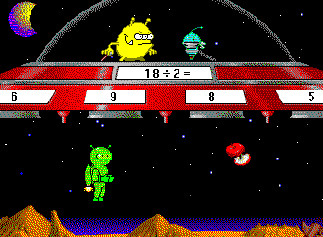
\includegraphics[scale=0.5,natwidth=296,natheight=217]{tics/math_blaster.jpg}
	\caption{Math Blaster, \emph{edutainment} del año 1987}
	\label{fig:math_blaster} 
\end{figure}

Los \emph{edutainment} fallaron en enseñar habilidades no triviales, se enfocan
principalmente enseñar tareas extremadamente repetitivas que no dependen de un
contexto\cite{charsky:2010}\cite{egenfeldt2007third}\cite{bruckman1999can}, son
excelentes para enseñar a sumar, pero no para aplicar ese conocimiento, analizar
y obtener conclusiones, o evaluar lo que aprendieron.

Las principales causas por las cuales los \emph{edutainment} fracasaron en su
intento de ser una alternativa viable a la educación son según
\cite{egenfeldt2007third}: 

\begin{description}

    \item[Falta de motivación interna] la única forma que tenían de intentar que
	    el alumno quiera seguir jugando eran las recompenzas, que eran muy
	    seguidas y fáciles de conseguir.

    \item[Aprendizaje como anexo] el principal objetivo del desarrollo de los
	    \emph{edutainment} eran el de entretener, los objetivos pedagógicos
	    eran agregados al final. Se enviaban informaciones al alumno
	    mediante largos textos que normalmente eran omitidos.
    
    \item[Jugabilidad sencilla] la mayoría eran sencillos juegos de arcade, la
	    mayor parte de la interacción eran a traves de palabras que eran
	    presentadas en forma de selección multiple. 

    \item[Ejercicios de prueba y error sistemáticos] todas las debilidades
	    anteriores se pueden fundamentar en el hecho de que los juegos
	    permitían al alumno intentar varías veces antes de dar una opción
	    correcta, sumando esto al echo de que los mismos no estaban
	    motivados, provocaba que todas las opciones sean probadas sin el
	    proceso de reflexión necesario para aprender, por ejemplo, varios
	    juegos aritméticos solicitaban pruebas del tipo
	    \begin{math}{2+2}\end{math} el alumno probaba diferentes resultados
	    y luego memorizaba el mismo. Se enseñaba a probar opciones sin
	    sentido antes que entender y analizar la experiencia.

\end{description}

\subsection{Entrenamiento basado en computadoras}

Cuando aparecieron en el mercado computadoras con multimedia, se argumento que
los ejercicios de la era anterior fallaron en su objetivo de una educación
profunda por que no contenían multimedia\cite{leinonen:ict}, las aplicaciones
eran distribuidas por CD-ROM, y así se actualizaban de manera más frecuente, y
podían contener gran cantidad de contenido multimedia.

Las bases pedagógicas de esta se basada en la capacidad de ciertos estudiantes
de aprender mejor cuando interactúan con contenido multimedia, la \emph{prueba y
	error} aún estaban presentes, pero no eran presentados inmediatamente,
sino más bien una vez que el alumno ya debería haber asimilado los conceptos y
funcionaban como pruebas de adquisición de conocimiento. Este tipo de contenido
tampoco logro la enseñanza profunda, solamente fueron efectivos en el
aprendizaje de idiomas, fallando en todos los demás campos\cite{leinonen:ict},
además los contenidos muchas veces estaban desactualizados y obtener nuevas
versiones no era una tarea sencilla.

Varios gobiernos apoyaron de manera agresiva la introducción de las \Gls{tic} en
educación\cite{mcdougall2006theory} y se realizo un importante avance teórico
con los trabajos sobre el aprendizaje construccionista de Papert y Harel (1991),
y la influencia de las computadoras sobre el aprendizaje y la mente de Marvin
Minksy (1987)~\cite{mcdougall2006theory}.

A comienzos de la decada de 1990, con la popularización de Internet, se le vio
como solución al problema de las poco frecuentes actualizaciones de aplicaciones
educativas, su utilización no tenia bases pedagógicas, más bien se basaban en la
facilidad de distribuir contenido por la \emph{Web}, el principal inconveniente
era la velocidad del Internet, no era suficiente para proveer entornos ricos en
multimedia como lo hacían los CD-ROM\cite{leinonen:ict}.

\begin{figure}[ht!] 
	\centering 
	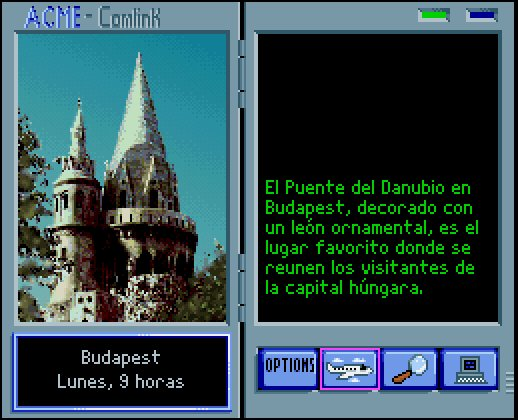
\includegraphics[scale=0.5]{tics/carmen.jpg}
	\caption{Donde en el mundo esta Carmen Sandiego} 
	\label{fig:carmen}
\end{figure}

Donde en el mundo esta Carmen Sandiego (ver~\ref{fig:carmen}) es un juego que
representa el potencial multimedia de esta época, el objetivo del juego era
detener a una serie de criminales mediante una serie de pistas que eran
provistas en forma de texto\cite{charsky:2010}. Este exitoso juego demuestra las
falencias de esta época, siendo visualmente muy atractivo, y con contenido
multimedia acorde a su tiempo, no era más que prueba y error, cada nivel del
juego podía ser completado sin leer el texto que contenía la información
educativa.

Todos los errores cometidos en la época anterior estaban presentes nuevamente,
no se establecieron marcos teóricos que fundamentasen la utilización de
contenido multimedia, así, se solucionaron los problemas de simplicidad, pero se
demostró que el principal problema era la prueba y error sistemático y sin
sentido\cite{egenfeldt2007third} 

\subsection{e-Learning}

La bases pedagógicas de esta son similares a la era del entrenamiento basado en
computadoras, se distribuye contenido masivamente a los alumnos, y luego, de
manera muy discreta se permite a los mismos colaborar, dejando siempre en claro
que primero se debe asimilar toda la información posible y luego relacionarse
con los demás\cite{leinonen:ict}.

\emph{E-Learning} se define como la educación y capacitación a traves de medios
digitales, incluye todo tipo de media capaz de distribuir información, puede ser
síncrono o asíncrono, y es particularmente útil para educación a distancia y con
horarios flexibles. Se origino a finales de la década de 1990 y tubo su apogeo a
mediados de la década del 2000, apoyada por la gran penetración de las \Gls{tic}
en la población\cite{punie:ict}.

Todos los paradigmas anteriores viven dentro del \emph{e-Learning}, permitiendo
compartir contenido multimedia y realizar pruebas del tipo \emph{prueba-error}. 

\begin{figure}[h] \centering 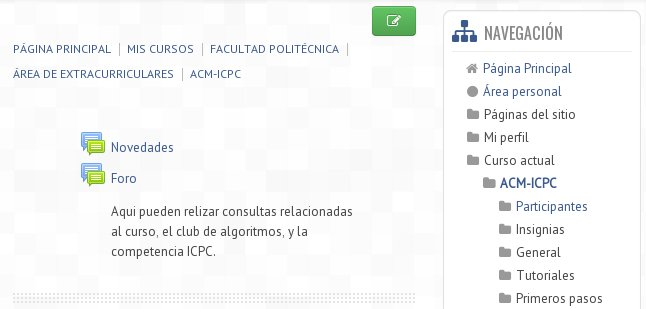
\includegraphics[scale=0.5]{tics/moodle.jpg}
	\caption{Moodle, plataforma de e Learning} \label{fig:moodle}
\end{figure}

La plataforma \emph{Moodle} (ver~\ref{fig:moodle}) cuya primera versión salio en
el 2002, es una de las principales herramientas del \emph{e-Learning} hoy en
día, permite la creación de cursos específicos por materia y sitios
especializados por instituciones académicas\cite{perkins2006using}. 

Si bien en las anteriores épocas, el uso de las \Gls{tic} estaba más orientado
hacia la educación básica y secundaría, el \emph{e-Learning} actualmente es más
utilizado en la educación terciaría\cite{punie:ict}.

La utilización del \emph{e-Learning} tiene varios grados de aplicación en
entornos reales\cite{punie:ict}, que van desde ser simples elementos
complementarios a la clase, como por ejemplo un repositorio para las
diapositivas y otros materiales de clase, hasta cursos completamente en linea,
donde la clase ha sido completamente sustituída.

